\begin{titlepage}
\begin{center}

% Upper part of the page. The '~' is needed because only works if a paragraph has started.

\includegraphics[width=0.35\textwidth]{./logo}~\\[1cm]

\textsc{\Large }\\[0.5cm]

% Title
\HRule \\[0.4cm]

{\huge \bfseries Problème à N-corps:\\
 algorithmes et parallélisations\\[0.4cm] }

\HRule \\[1.5cm]

% Author and supervisor

\begin{center}
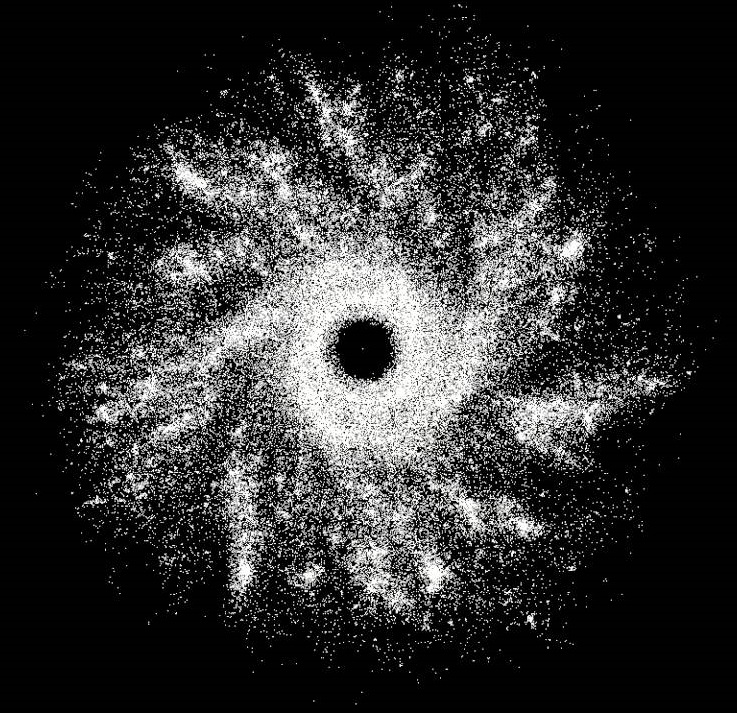
\includegraphics[width=0.5\textwidth]{./galaxy.jpg}~\\[1cm]
\end{center}
\begin{minipage}{0.4\textwidth}
\begin{flushleft} \large
\emph{Auteurs:}\\
Rudio \textsc{FIDA CYRILLE}\\
Noah \textsc{VEYTIZOUX}\\
Elyas \textsc{Assili}\\
Camille \textsc{Hascoet}
\end{flushleft}
\end{minipage}
\begin{minipage}{0.4\textwidth}
\begin{flushright} \large
\emph{Référent:} \\
Roméo \textsc{MOLINA}
\end{flushright}
\end{minipage}

\vfill

% Bottom of the page
{\large \today}

\end{center}
\end{titlepage}
